%% LyX 2.3.5.2 created this file.  For more info, see http://www.lyx.org/.
%% Do not edit unless you really know what you are doing.
\RequirePackage{fixltx2e}
\documentclass[11pt,aspectratio=169]{beamer}
\usepackage{lmodern}
\usepackage{lmodern}
\usepackage[T1]{fontenc}
\usepackage[utf8]{inputenc}
\setcounter{secnumdepth}{0}
\setcounter{tocdepth}{3}
\usepackage{amstext}
\usepackage{amsthm}
\usepackage{amssymb}
\usepackage{graphicx}

\makeatletter
%%%%%%%%%%%%%%%%%%%%%%%%%%%%%% Textclass specific LaTeX commands.
% this default might be overridden by plain title style
\newcommand\makebeamertitle{\frame{\maketitle}}%
% (ERT) argument for the TOC
\AtBeginDocument{%
  \let\origtableofcontents=\tableofcontents
  \def\tableofcontents{\@ifnextchar[{\origtableofcontents}{\gobbletableofcontents}}
  \def\gobbletableofcontents#1{\origtableofcontents}
}

\@ifundefined{date}{}{\date{}}
%%%%%%%%%%%%%%%%%%%%%%%%%%%%%% User specified LaTeX commands.
%\usetheme{metropolis}
%\usetheme{Darmstadt}
\usetheme{default}
\setbeamertemplate{navigation symbols}{}

\usepackage[bottom]{footmisc}
\usepackage{placeins}
%\usepackage[adobe-utopia]{mathdesign}
\usepackage{pifont}
%\usepackage{kerkis}
%\usepackage{pxfonts}
\usepackage[default]{lato}
%\usepackage{mathpazo}
\usepackage{eulervm}
\usepackage{animate}


\usepackage{dcolumn}
\usepackage{bbm}
\newcolumntype{d}[0]{D{.}{.}{5}}

\usepackage{changepage}

\addtobeamertemplate{frametitle}{}{\vspace{-0.2 cm}}

\setbeamertemplate{frametitle} 
{ 
	\begin{centering} 
		\LARGE
		\insertframetitle
		\par 
	\end{centering} 
} 

\setbeamerfont{title}{size = \LARGE}





%COLORS
\definecolor{chamois}{RGB}{254,254,245}
\definecolor{oldchamois}{RGB}{255,255,240}
\definecolor{darkbrown}{RGB}{124,79,0}
\definecolor{UniBlue}{RGB}{65,55,203}
\definecolor{bordeaux}{RGB}{201,18,18}
\definecolor{redd}{RGB}{245,29,29}


\definecolor{hellgelb}{rgb}{1,1,0.8}
\definecolor{colKeys}{rgb}{0,0,1}
\definecolor{colIdentifier}{rgb}{0,0,0}
\definecolor{colComments}{rgb}{1,0,0}
\definecolor{colString}{rgb}{0,0.5,0}
\definecolor{textcolour}{rgb}{0.37,0.34,0.27}

\definecolor{ITgreen}{rgb}{0,204/256,0}

\iffalse
%LIN AT THE TOP
\usepackage{tikz}
\newcommand{\topline}{%
	\tikz[remember picture,overlay] {%
		\draw[bordeaux,thick] ([yshift=-1.4cm]current page.north west)-- ([yshift=-1.4cm,xshift=\paperwidth]current page.north west);}}

\addtobeamertemplate{frametitle}{
}{\topline%
}
\fi

%ITEMIZE SEP
\setlength{\itemsep}{10mm}
%BACKGROUND AND ITEMIZE
%\setbeamercolor{background canvas}{bg=chamois}
\setbeamercolor{itemize item}{fg=bordeaux}
%\setbeamertemplate{itemize item}{\maltese}
\setbeamercolor{itemize subitem}{fg=bordeaux}
\setbeamertemplate{itemize subitem}{$\diamondsuit$}

%ELEMENT COLORS
\setbeamercolor{title}{fg=UniBlue}
\setbeamercolor{frametitle}{fg=UniBlue}
\setbeamercolor{structure}{fg=textcolour}

%COLORS FIRST PAGE
\setbeamercolor{author}{fg=darkbrown}
\setbeamercolor{date}{fg=darkbrown!60}
\setbeamercolor{institute}{fg=darkbrown}

%BLOCK SPECS
\setbeamercolor{block title}{bg=UniBlue!30,fg=white}
\setbeamercolor{block body}{bg=UniBlue!10,fg=black}
%\addtobeamertemplate{block begin}{%
%	\centering
%	\setlength{\textwidth}{1\textwidth}%
%}{}

%\setbeamercolor{block title alerted}{bg=yellow!60,fg=red}
%\setbeamercolor{block body alerted}{bg=hellgelb!80,fg=UniBlue}


\setbeamercolor{alert}{fg=redd}
\renewcommand<>{\alert}[1]{%
	{\usebeamercolor[fg]{alert}\only#2{}#1}%
}

\newcommand{\blue}{\color{blue}}






\usepackage{tabularx}
\usepackage{booktabs}
\usepackage{epstopdf}
\usepackage{graphicx}



\newcolumntype{C}[1]{>{\centering\let\newline\\\arraybackslash\hspace{0pt}}m{#1}}
\newcolumntype{L}[1]{>{\flushleft\let\newline\\\arraybackslash\hspace{0pt}}m{#1}}
\newcolumntype{P}{>{\centering\arraybackslash}m{3cm}}
\renewcommand{\baselinestretch}{1.3} 
\usepackage{lscape}

%%% TIKZ %%%%
\usepackage{tikz}
\usetikzlibrary{positioning}
\usetikzlibrary{snakes}
\usetikzlibrary{calc}
\usetikzlibrary{arrows}
\usetikzlibrary{decorations.markings}
\usetikzlibrary{shapes.misc}
\usetikzlibrary{matrix,shapes,arrows,fit,tikzmark}
\usepackage{pgfplots}

\setbeamertemplate{footnote}{%
\insertfootnotemark\footnotesize\insertfootnotetext\par%
}



\usepackage{dcolumn}
\usepackage{bbm}
\newcolumntype{d}[0]{D{.}{.}{1}}
\newcolumntype{C}[1]{>{\centering\let\newline\\\arraybackslash\hspace{0pt}}m{#1}}
\newcolumntype{L}[1]{>{\flushleft\let\newline\\\arraybackslash\hspace{0pt}}m{#1}}
\newcolumntype{P}{>{\centering\arraybackslash}m{3cm}}
\renewcommand{\baselinestretch}{1.3} 

\newcolumntype{H}{>{\setbox0=\hbox\bgroup}c<{\egroup}@{}}
\usepackage{}

\makeatother

\begin{document}
\title{14.661 Recitation 4: LCLS under Uncertainty}
\author{Andrea Manera\footnote[frame]{I thank Clémence Idoux for sharing her material with me. All remaining errors are my own.}}
\date{Fall 2021}

\makebeamertitle
%
\begin{frame}

\frametitle{Road map}
\begin{itemize}
\item Theory of LCLS under uncertainty
\item Altonji (1986)
\end{itemize}
\end{frame}
%
\begin{frame}{LCLS under uncertainty - Set up}

Additively separable utility function: 
\begin{eqnarray*}
\sum_{s=t}^{T}\frac{1}{1+\rho}^{s-t}U(c_{s},h_{s})
\end{eqnarray*}
\pause

Intertemporal budget constraint: 
\begin{eqnarray*}
A_{t+1}=(1+r_{t})A_{t}+w_{t}h_{t}-c_{t}
\end{eqnarray*}
\pause Uncertainty: add expectation operator in front of what seen
in class: 
\begin{eqnarray*}
\max_{\left\lbrace h_{t},c_{t}\right\rbrace _{s=t}^{T}}E_{t}\left[\sum_{s=t}^{T}\left(\frac{1}{1+\rho}\right)^{s-t}U(c_{s},h_{s})\right]\\
\textrm{s.t }A_{t+1}=(1+r_{t})A_{t}+w_{t}h_{t}-c_{t}
\end{eqnarray*}

\end{frame}
%
\begin{frame}{Solving the problem}
\begin{itemize}
\item From 14.451, with concave utility and exponential discounting, we
can:\pause
\end{itemize}
\begin{enumerate}
\item Use a variational approach, find the asset path that satisfies Euler
equation and transversality\pause
\item Set up the problem recursively, and walk down Bellman's road\pause
\end{enumerate}
\begin{itemize}
\item They give the same solution in this context, as the conditions for
the ``sufficiency theorem'' hold (see Alp's 14.661 notes and Daron's
book ``Introduction to Modern Economic Growth''):\pause
\begin{itemize}
\item Strict concavity of objective function in the control and state variable;\pause
\item Differentiability (we assume it);\pause
\item The state variable has a lower bound and objective increases in the
state.
\end{itemize}
\end{itemize}
\end{frame}
%
\begin{frame}{Bellman equation}

By the above conditions, let's solve the problem 
\begin{align*}
V_{t}(A_{t}|\mathcal{I}_{t})= & \max_{h_{t},c_{t}}U(c_{t},h_{t})+\frac{1}{1+\rho}E_{t}V_{t+1}(A_{t+1}|\mathcal{I}_{t+1})\\
\text{s.t.} & \ A_{t+1}=(1+r_{t})A_{t}+w_{t}h_{t}-c_{t}
\end{align*}
\pause
\begin{itemize}
\item $V_{t}(A_{t}|\mathcal{I}_{t})$ is the optimum value function given
available information in $t$, $\mathcal{I}_{t}$ \pause
\begin{itemize}
\item State variable is accumulated assets at time $t,\ A_{t},$
\item The constraint is the law of motion of the agent's assets
\end{itemize}
\end{itemize}
\end{frame}
%
\begin{frame}{FOCs}

Replacing $A_{t+1}=(1+r_{t})A_{t}+w_{t}h_{t}-c_{t}$ in the Bellman
equation, we can get the following f.o.c.'s \pause
\begin{eqnarray}
c_{t}:\quad U_{c}(c_{t},h_{t})-\frac{1}{1+\rho}E_{t}[V_{t+1}'(A_{t+1})] & = & 0\\
h_{t}:\quad U_{h}(c_{t},h_{t})+\frac{1}{1+\rho}w_{t}E_{t}[V_{t+1}'(A_{t+1})] & = & 0
\end{eqnarray}
\pause

To solve the problem, we also add the \emph{envelope condition}: 
\begin{eqnarray}
A_{t}:\quad V_{t}'(A_{t})=\frac{1}{1+\rho}(1+r_{t})E_{t}[V_{t+1}'(A_{t+1})]\label{ET}
\end{eqnarray}
\pause This relates the MU of wealth today to the expected MU of wealth
tomorrow
\end{frame}
%
\begin{frame}

\frametitle{MU of wealth}

Define the MU of wealth at time $t$: 
\begin{eqnarray*}
\lambda_{t}\equiv V_{t}'(A_{t}|\mathcal{I}_{t})
\end{eqnarray*}
Then \eqref{ET} gives: 
\begin{eqnarray*}
\lambda_{t}=\frac{1+r_{t}}{1+\rho}E_{t}[\lambda_{t+1}]
\end{eqnarray*}
\end{frame}
%
\begin{frame}

\frametitle{Euler equations}

Plugging in we get two Euler equations: 
\begin{align}
U_{c}(c_{t},h_{t}) & =\frac{1}{1+r_{t}}\lambda_{t}=E_{t}\left[\frac{1+r_{t+1}}{1+\rho}U_{c}(c_{t+1},h_{t+1})\right]\label{MUC}\\
U_{h}(c_{t},h_{t}) & =-\frac{w_{t}}{1+r_{t}}\lambda_{t}=E_{t}\left[\frac{1+r_{t+1}}{1+\rho}\frac{w_{t}}{w_{t+1}}U_{h}(c_{t+1},h_{t+1})\right]\label{MUL}
\end{align}
\pause

As in class with one difference.
\begin{itemize}
\item $\lambda_{t}$ is no longer time invariant : 
\[
\lambda_{t}=\frac{1+r_{t}}{1+\rho}E_{t}\left[\lambda_{t+1}\right]=E_{t}\left[\Pi_{s=t}^{T-1}\frac{1+r_{s}}{1+\rho}\lambda_{T}\right]
\]
\pause
\item summarizes the expected path of the MU of wealth in all future periods
given current information
\end{itemize}
\end{frame}
%
\begin{frame}

\frametitle{Deriving the HeckMaC LS Equation}

Assuming a HeckMaC separable utility function:
\[
U\left(c_{t},h_{t}\right)=c_{t}^{\delta_{1}}-\gamma_{2}h_{t}^{\delta_{2}}
\]
 and taking logarithms of the FOC, we can define the ISE

\begin{equation}
\ln h_{t}=\Big[\frac{\ln\lambda_{t}-\ln\gamma_{2}-\ln\delta_{2}}{\delta_{2}-1}\Big]+\frac{t}{\delta_{2}-1}\ln\Big(\frac{1+\rho}{1+r_{t}}\Big)+\underbrace{\frac{1}{\delta_{2}-1}}_{\equiv\delta\text{ (ISE)}}\ln w_{t}\label{key}
\end{equation}
\pause

How do we take first differences to eliminate $\lambda_{t}$?\pause
\begin{itemize}
\item By definition:
\[
\lambda_{t+1}=E_{t}[\lambda_{t+1}]+\epsilon_{t+1}
\]
\item Assuming rational expectation, $\epsilon_{t+1}$ is orthogonal to
information available at $t$\pause
\end{itemize}
\end{frame}
%
\begin{frame}

\frametitle{HeckMaC Estimation with Uncertainty}

\begin{eqnarray*}
\frac{1+\rho}{1+r_{t}}\lambda_{t} & = & E_{t}[\lambda_{t+1}]\\
 & = & \lambda_{t+1}-\epsilon_{t+1}
\end{eqnarray*}

\pause
\begin{itemize}
\item $\ln\lambda_{t}$ obtained taking logs and using Taylor expansion
around $\epsilon_{t+1}=0$ 
\begin{align*}
\ln\lambda_{t}+\ln\Big(\frac{1+r_{t}}{1+\rho}\Big) & =\ln\left(\lambda_{t+1}-\epsilon_{t+1}\right)-\ln\lambda_{t+1}+\ln\lambda_{t+1}\\
 & \approx\ln\lambda_{t+1}+\underset{\equiv u_{t}}{\underbrace{\frac{1}{\lambda_{t+1}}\left(-\epsilon_{t+1}\right)}}
\end{align*}
\end{itemize}
\end{frame}
%
\begin{frame}

\frametitle{Consistency of ISE estimates I}

Taking first differences we get rid of $\lambda_{t}$\pause\medskip{}

\begin{equation}
\Delta\ln h_{it}=\gamma+\mu_{i}+\delta\Delta\ln w_{it}+\delta\Delta u_{it}+e_{it}\label{key}
\end{equation}

BUT we still have the term $u_{it}$ after differencing

\medskip{}

To get a consistent estimator of the ISE $\delta=\frac{1}{\delta_{2}-1}$
, need $cov(u_{it},\ln{w_{it}})=0$ for all individuals.\pause
\begin{itemize}
\item Altonji (1986): reasonable if individuals know wages one period in
advance and have rational expectation 
\item $\epsilon_{t+1}$ is orthogonal to information in period $t$, so
uncorrelated with time-$t$ variables like $\ln{w_{it}}$.
\end{itemize}
\end{frame}
%
\begin{frame}

\frametitle{Consistency of ISE estimates II}

\begin{eqnarray*}
cov(u_{it},\ln{w_{t}}) & = & E_{t}(u_{it}\ln{w_{t}})-E_{t}(u_{it})E_{t}(\ln{w_{it}})\\
 & = & E_{t}\Big(\frac{(1+r_{t})\epsilon_{it+1}}{(1+\rho)\lambda_{t}}\ln{w_{it}}\Big)\\
 & = & \frac{1+r_{t}}{(1+\rho)\lambda_{t}}E_{t}(\epsilon_{it+1}\ln{w_{it}})\\
 & = & 0
\end{eqnarray*}
\pause
\begin{itemize}
\item First line uses definition of covariance, 
\item Second line uses definition of $u_{it}$ and the fact that $E_{t}(u_{it})=\frac{1+r_{t}}{(1+\rho)\lambda_{t}}E_{t}(\epsilon_{it+1})$
, 
\item Third line uses the fact that $\lambda_{t}$ and $r_{t}$ is a constant
in period $t$
\item Last line from RE: orthogonality of error terms
\end{itemize}
\end{frame}
%
\begin{frame}

\frametitle{Altonji (1986) - Introduction}
\begin{itemize}
\item \textbf{Aim of the paper: }Estimate the ISE given by the HeckMcCurdy
regression

\begin{equation}
\ln h_{t}=\Big[\frac{\ln\lambda_{t}-\ln\gamma_{2}-\ln\delta_{2}}{\delta_{2}-1}\Big]+\frac{t}{\delta_{2}-1}\ln\Big(\frac{1+\rho}{1+r_{t}}\Big)+\underbrace{\frac{1}{\delta_{2}-1}}_{\equiv\delta\text{ (ISE)}}\ln w_{t}\label{key}
\end{equation}
\pause
\item \textbf{Data:} PSID with its March supplement\pause
\item \textbf{Main identification challenge:} \pause
\begin{itemize}
\item Labor supply depends both on current wages $w_{it}$ and on the all
past and future wages through the marginal utility of wealth $\lambda_{it}$
\pause
\item Can control for it through labor supply in previous periods (i.e using
Fixed Effects) 
\item But this exacerbates measurement error in wages 
\end{itemize}
\end{itemize}
\end{frame}
%
\begin{frame}

\frametitle{Altonji (1986) - Empirical strategy}

\textbf{Approach 1 to control for $\lambda_{it}$: Use of past labor
as proxy for $\ln\lambda_{it}$}\pause
\begin{itemize}
\item similar to MaCurdy but does not assume perfect foresight (i.e. use
LCLS with uncertainty) \pause
\item Instead, assume rational expectation and knowledge of $w_{it}$ one
period in advance which we showed leads to the same estimation equation
\pause
\item Use a second measure for wage (the direct answer to the march survey
question about hourly wage) as an instrument for wage to solve the
measurement error problem 
\end{itemize}
\end{frame}
%
\begin{frame}

\frametitle{Altonji (1986) - Empirical strategy}

\textbf{Approach 2 to control for $\lambda_{it}$: Use of consumption
as a proxy for $\ln\lambda_{it}$}\pause
\begin{itemize}
\item FOC for consumption \eqref{MUC} gives $\ln\lambda_{it}$ as a function
of $c_{it}$. Use consumption to hold constant marginal utility of
wealth \pause
\item Note that it works because separability of the utility function implies
that consumption depends on current wages $w_{it}$ only through $\ln\lambda_{it}$
\pause
\item in practice, instruments both wage and consumption with the additional
measure of wage and the permanent component of wage 
\end{itemize}
\end{frame}
%
\begin{frame}

\frametitle{Altonji (1986) - Empirical strategy}

\textbf{Pros and Cons of the 2nd approach VS 1st approach:} \pause
\begin{itemize}
\item Pros: does not require to add FE and so keeps a lot of variation and
minimize measurement error problem 
\item Pros: does not require perfect foresight or rational expectation \pause
\item Cons: assume no unobserved differences in preferences for labor supply/consumption
between individuals 
\item Cons: requires separability of preferences (whereas FD can be seen
as log-linear approximation of true demand system) 
\end{itemize}
\end{frame}
%
\begin{frame}

\frametitle{Altonji (1986) - Approach 1 results}

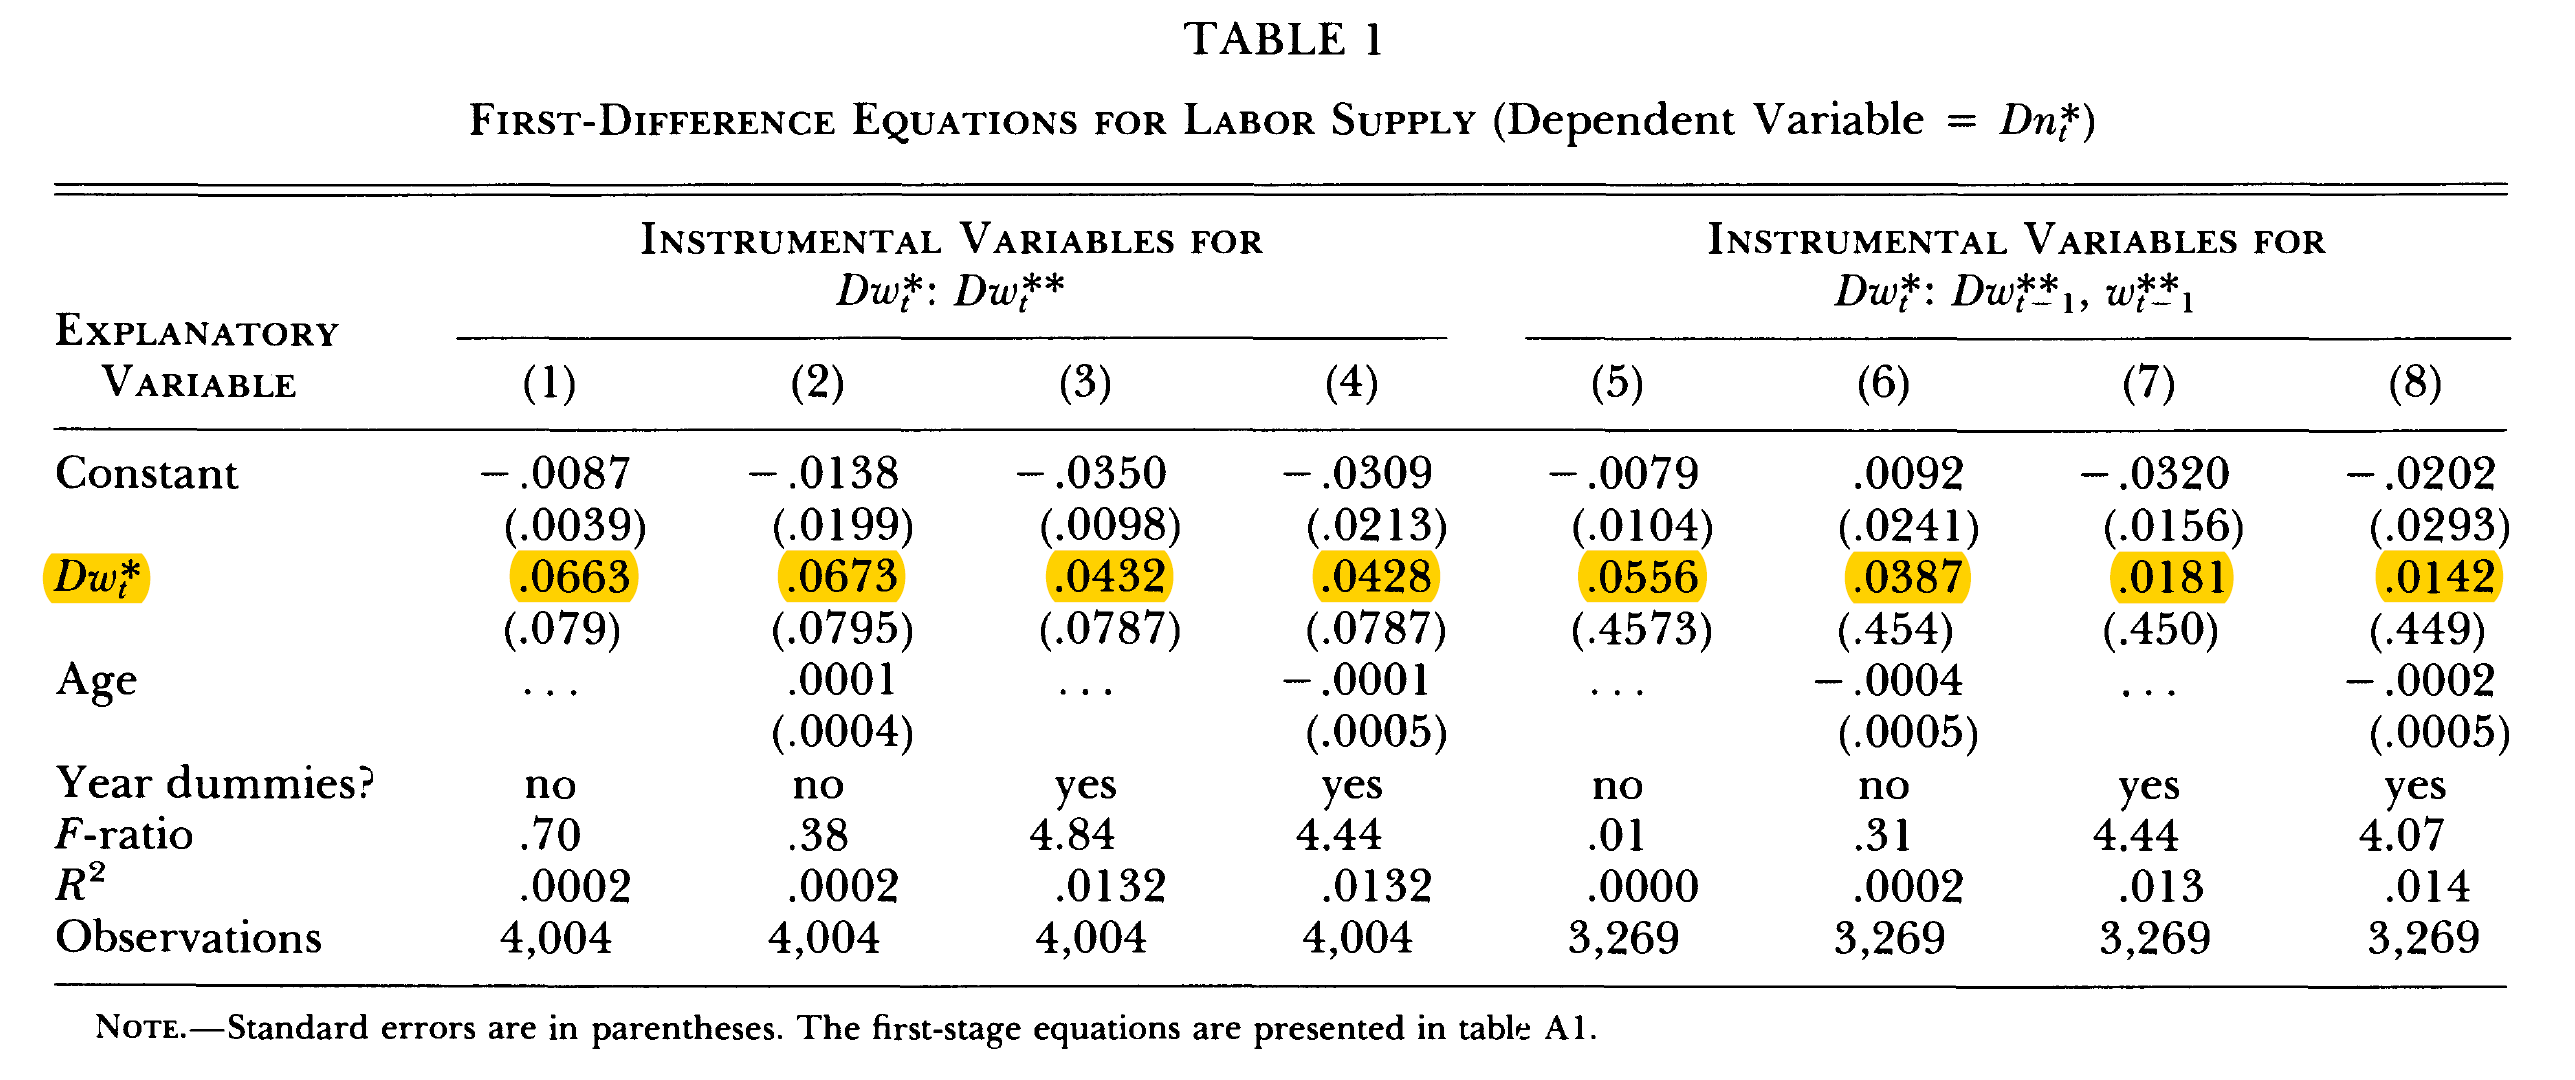
\includegraphics[width=1\textwidth]{Altonji1} 
\end{frame}
%
\begin{frame}

\frametitle{Altonji (1986) - Approach 2 results}

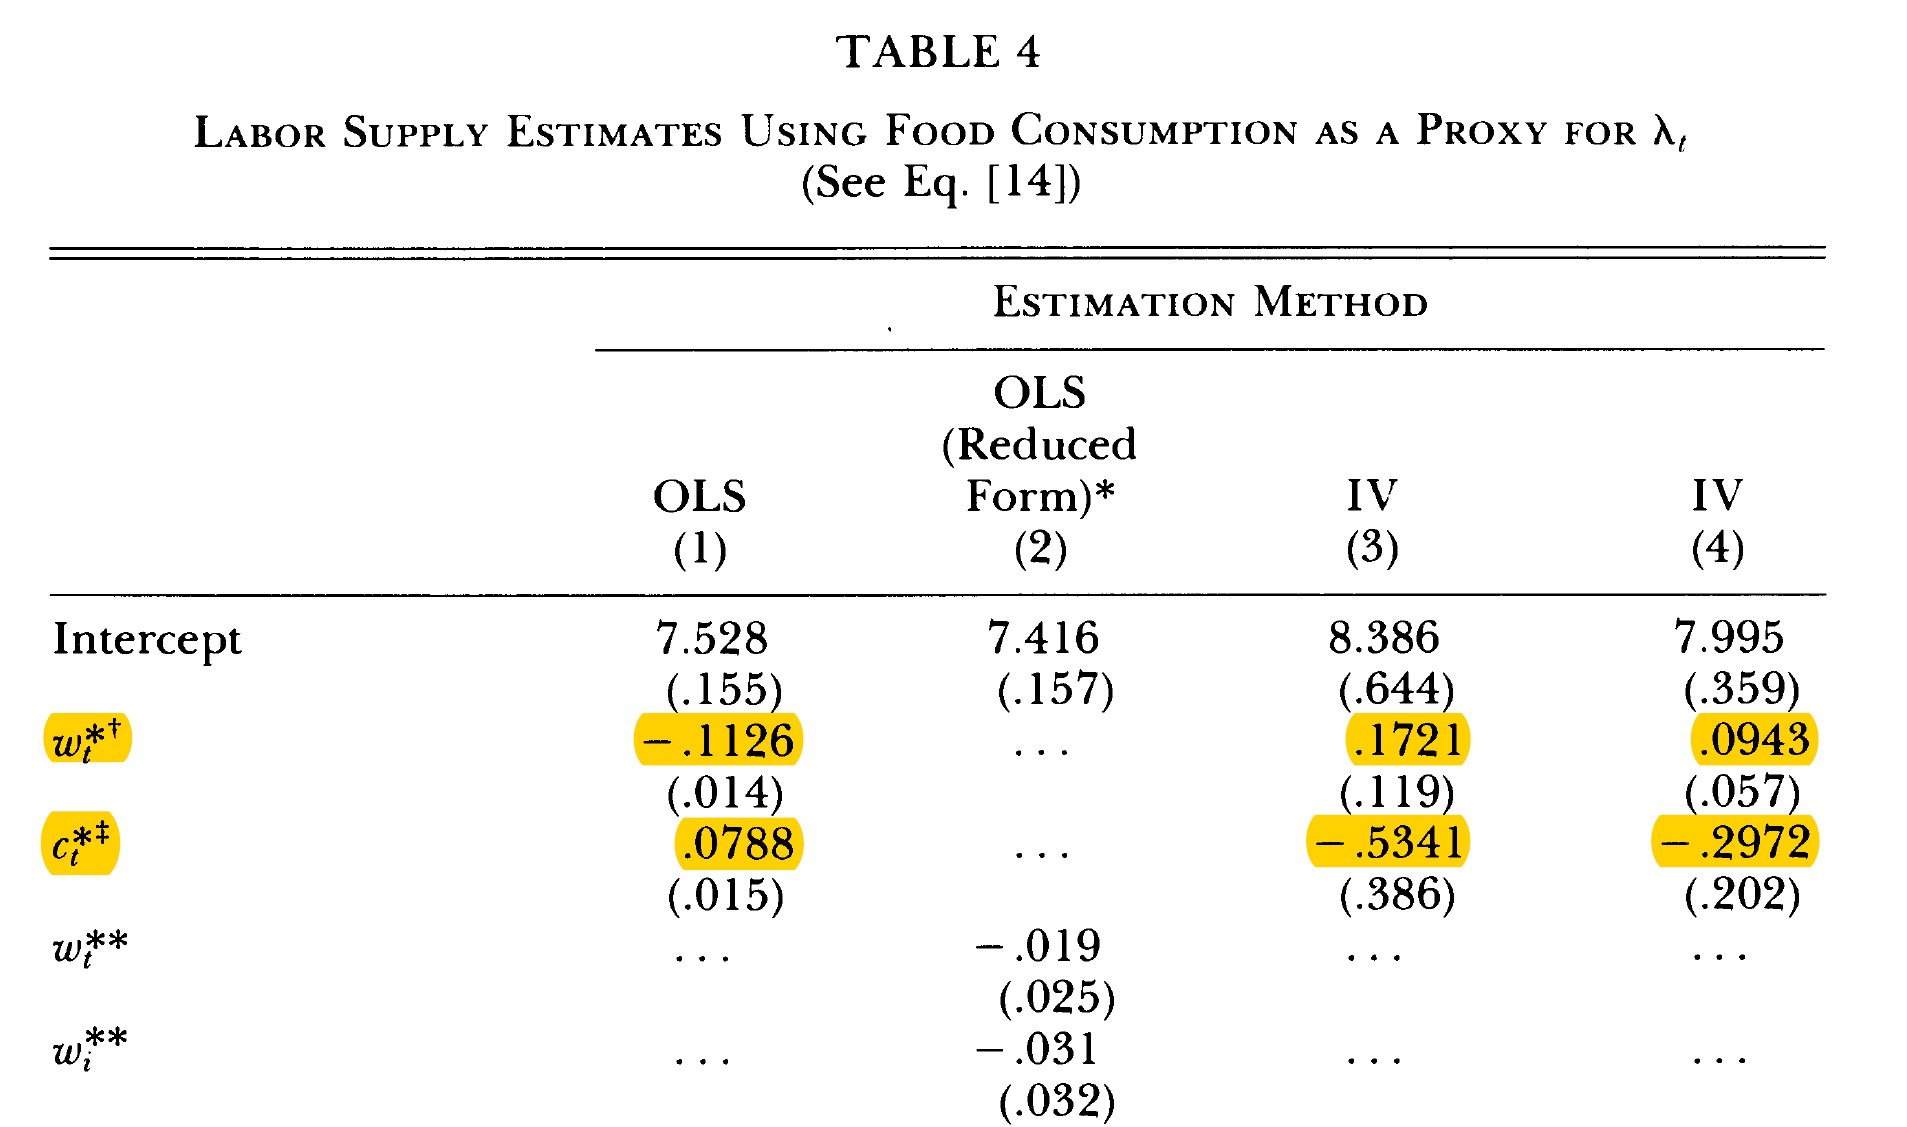
\includegraphics[width=0.9\textwidth]{Altonji2} 
\end{frame}
%
\begin{frame}

\frametitle{Altonji (1986) - Conclusions}
\begin{itemize}
\item Estimates of ISE between 0.01 and 0.1721 : quite small and similar
to MaCurdy. \pause
\item \textbf{Main concern:} non-separable preferences lead to an upward
bias in the ISE from the consumption approach. 
\item In this case, $\ln w_{it}$ enters in the consumption FOC.
\end{itemize}
\end{frame}

\end{document}
